\documentclass[12pt, twoside]{article}
\usepackage[letterpaper, margin=1in, headsep=0.5in]{geometry}
\usepackage[english]{babel}
\usepackage[utf8]{inputenc}
\usepackage{amsmath}
\usepackage{amsfonts}
\usepackage{amssymb}
\usepackage{tikz}
\usetikzlibrary{quotes, angles}
\usepackage{graphicx}
\usepackage{enumitem}
\usepackage{multicol}

\newif\ifmeta
\metatrue %print standards and topics tags

\title{Regents Geometry}
\author{Chris Huson}
\date{September 2020}

\usepackage{fancyhdr}
\pagestyle{fancy}
\fancyhf{}
\renewcommand{\headrulewidth}{0pt} % disable the underline of the header
\raggedbottom


\fancyhead[LE]{\thepage}
\fancyhead[RO]{\thepage \\ Name: \hspace{4cm} \,\\}
\fancyhead[L]{BECA / Dr. Huson / Geometry 06-Analytic-geometry\\* pset ID: 87}

\begin{document}

\subsubsection*{6-7DNQ-Distance+slope}
\begin{enumerate}
\item Write down the slope perpendicular to the given slope.
  \begin{enumerate}
    \begin{multicols}{2}
    \item   $m= \frac{2}{3} \hspace{1cm} m_{\perp} = $ \vspace{1cm}
    \item   $m= -2 \hspace{1cm} m_{\perp} = $
    \item   $m= 0.25 \hspace{1cm} m_{\perp} = $ \vspace{1cm}
    \item   $m= -\frac{1}{5} \hspace{1cm} m_{\perp} = $
    \end{multicols}
  \end{enumerate} \vspace{1cm}

  
\item The line $l$ has the equation $y=\frac{5}{2} x+9$.
  \begin{enumerate}
    \item What is the slope of the line $k$, given $k \parallel l$?
    \vspace{1.5cm}
    \item What is the slope of the line $j$, given $j \perp l$?
    \vspace{1.5cm}
  \end{enumerate}

\item What is the slope of a line parallel to the line $2x+2y=14$?  \vspace{4cm}
\item What is the slope of a line perpendicular to the line $-2x+y=1$?  
 
\newpage
    Note: The formula for distance is $\displaystyle d=\sqrt{(x_2-x_1)^2+(y_2-y_1)^2}$

\item Graph and label $\triangle ABC$ and find the lengths of its sides. $A(1,2)$, $B(9,8)$, $C(9,2)$.
    \begin{enumerate}
      \begin{multicols}{2}
      \item   $AC=$ \vspace{1.7cm}
      \item   $BC=$ \vspace{1.7cm}
      \item   $AB=$ \vspace{3cm}
        \begin{center}
          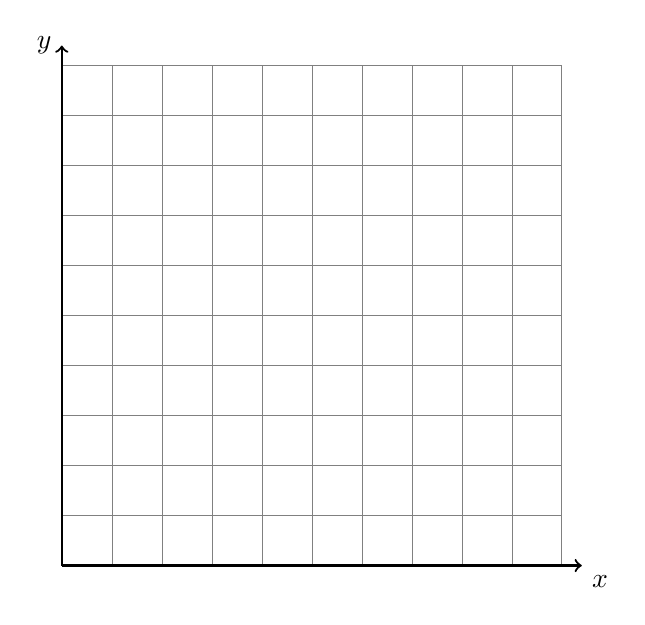
\begin{tikzpicture}[scale=.635]
            \draw [help lines] (0,0) grid (10,10);
            \draw [thick, ->] (0,0) -- (10.4,0) node [below right] {$x$};
            \draw [thick, ->] (0,0)--(0,10.4) node [left] {$y$};
          \end{tikzpicture}
          \end{center}
      \end{multicols}
    \end{enumerate}
    \vspace{1cm}

\item Find $c$. \hspace{8cm}
    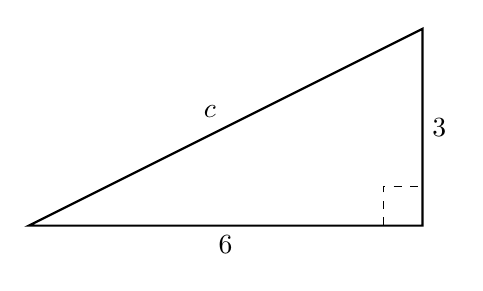
\begin{tikzpicture}[scale=1.25]
      \node at (2,1)[above left]{$c$};
      \node at (4,1)[right]{3};
      \node at (2,0)[below]{6};
      \draw [thick] (0, 0)--(4, 0)--(4, 2)--cycle;
      \draw [dashed] (4,0)++(-0.4,0)-- ++(0,0.4)-- +(0.4,0);
    \end{tikzpicture} \vspace{3cm}

\item What is the length of $\overline{CD}$ if $C(3,-1)$ and $D(-2,11)$?
      
\newpage
\item Graph and label the two equations. Mark their intersection as an ordered pair.
    \begin{multicols}{2}
      $y = x+7$ \\
      $4x+5y=-10$
    \end{multicols}     \vspace{2cm}
    Are the lines parallel, perpendicular, or neither? Justify your answer.
    \vspace{2cm}

    \begin{center} %4 quadrant regents grid w T-Chart
    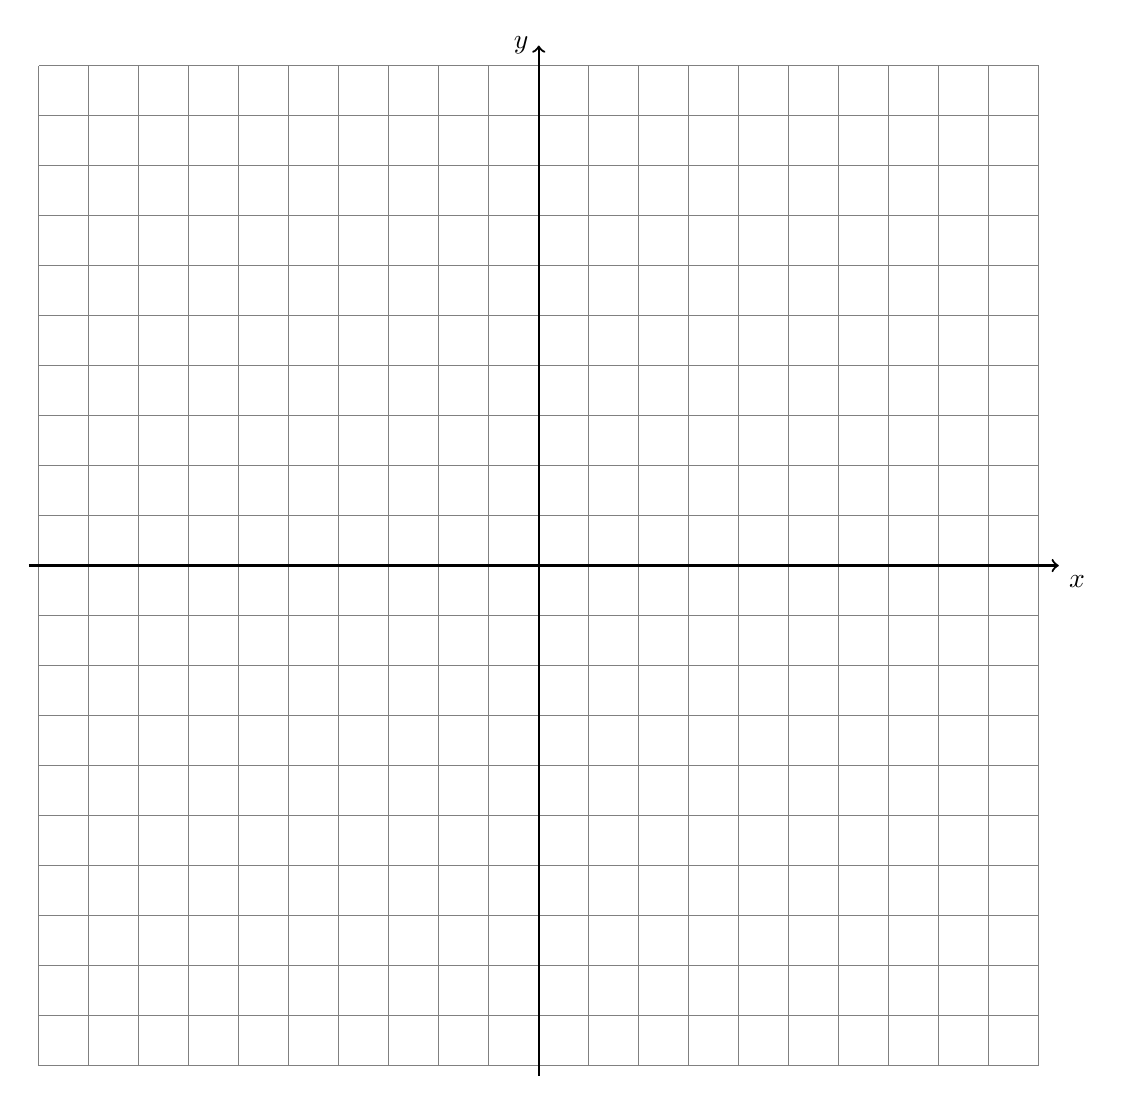
\begin{tikzpicture}[scale=.635]
      \draw [help lines] (-10,-10) grid (10,10);
      \draw [thick, ->] (-10.2,0) -- (10.4,0) node [below right] {$x$};
      \draw [thick, ->] (0,-10.2)--(0,10.4) node [left] {$y$};
    \end{tikzpicture}
    \end{center}

\newpage
\item On the graph below, draw $\overline{AB}$, with $A(-2,3)$ and $B(5,1)$, labeling the end points. Determine and state the coordinates of the midpoint $M$ of $\overline{AB}$ and mark and label it on the graph.
  \begin{flushright}
    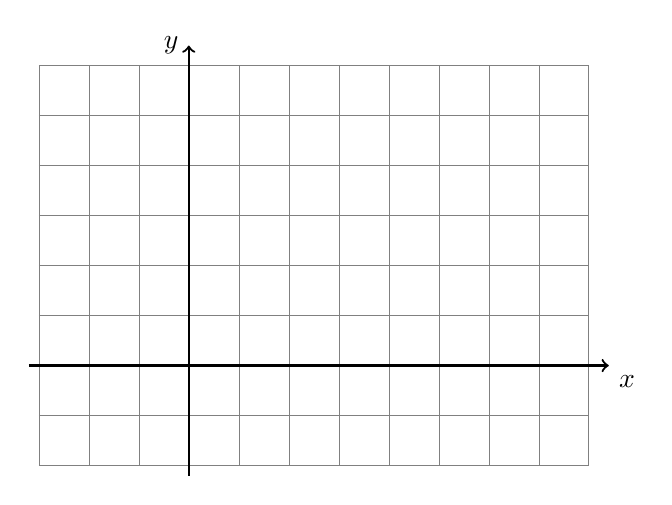
\begin{tikzpicture}[scale=.635]
      \draw [help lines] (-3,-2) grid (8,6);
      \draw [thick, ->] (-3.2,0) -- (8.4,0) node [below right] {$x$};
      \draw [thick, ->] (0,-2.2)--(0,6.4) node [left] {$y$};
    \end{tikzpicture}
  \end{flushright}
  \vspace{1cm}

\item Spicy: On the set of axes below, graph the quadrilateral $ABCD$ having coordinates $A(-3,-3)$, $B(5,1)$, $C(6,8)$, and $D(-2,4)$. Find the slope of each of the four sides. What type of quadrilateral is $ABCD$? Justify your answer.
    \begin{flushright} %4 quadrant regents grid
      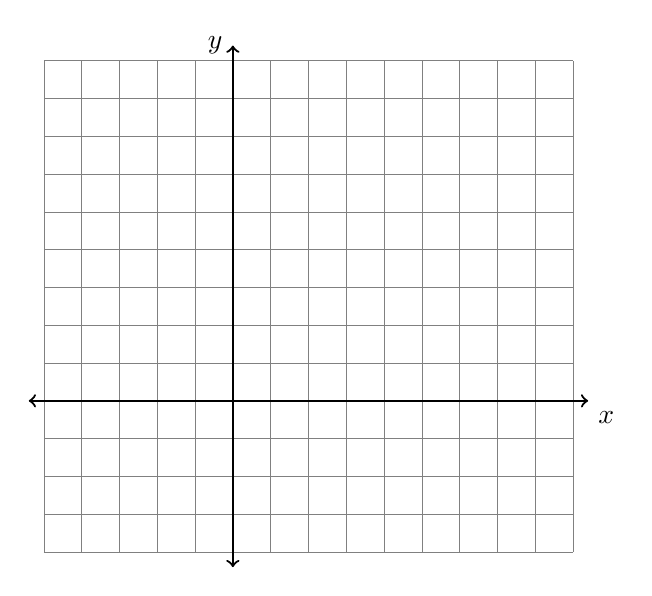
\begin{tikzpicture}[scale=.48]
        \draw [help lines] (-5,-4) grid (9,9);
        \draw [thick, <->] (-5.4,0) -- (9.4,0) node [below right] {$x$};
        \draw [thick, <->] (0,-4.4)--(0,9.4) node [left] {$y$};
        %\draw [thick] (-3,-3) node[below] {$A$}--
        %(5,1) node[right] {$B$}--
        %(6,8) node[right] {$C$}--
        %(-2,4) node[left] {$D$}--cycle;
        %\draw [fill] (5,0) circle [radius=0.1] node[above left] {$P$};
      \end{tikzpicture}
    \end{flushright}
    

\end{enumerate}
\end{document}